\documentclass{article}
\usepackage[utf8]{inputenc}
\usepackage{graphicx}
\usepackage{amsmath}
\usepackage{amssymb}
\usepackage{amsthm}

\title{Computational Physics (physics760)\\Exercise 3}
\author{Ajay S. Sakthivasan, Dongjin Suh}
\date{November 18, 2022}

\begin{document}

\maketitle

\section{Applying HMC to the long-range Ising model}

\begin{enumerate}
\item Derive expressions for O$[\phi]$ for mean magnetization (per site) and energy (per site)

\begin{flalign*}
Z[J > 0] &= \int_{-\infty}^{\infty} \frac{d\phi}{\sqrt{2\pi \beta J}} \mathrm{e}^{-\frac{\phi^2}{2\beta J} +N\log(2\cosh{(\beta h \pm \phi)})} &\\
&\\
\langle O\rangle &= \frac{1}{\mathrm{Z}} \int_{}^{} \frac{d\phi}{\sqrt{2\pi \beta J}} O[\phi] \mathrm{e}^{-S[\phi]}&\\
&\\
&\textbf{Mean Magnetization:} &\\
\langle m\rangle &= \frac{1}{N\beta} \frac{\partial}{\partial h} \log (\mathrm{Z}) &\\
\langle m\rangle &= \frac{1}{N\beta} \frac{\partial}{\partial h} \log\left( \int_{-\infty}^{\infty} \frac{d\phi}{\sqrt{2\pi \beta J}} \mathrm{e}^{-\frac{\phi^2}{2\beta J} +N\log(2\cosh{(\beta h \pm \phi)})}\right) &\\
&= \frac{1}{N\beta} \frac{1}{\mathrm{Z}} \int_{-\infty}^{\infty} \frac{d\phi}{\sqrt{2\pi \beta J}} \frac{\partial}{\partial h} \mathrm{e}^{-\frac{\phi^2}{2\beta J} +N\log(2\cosh{(\beta h \pm \phi)})}&\\
&= \frac{1}{N\beta} \frac{1}{\mathrm{Z}} \int_{-\infty}^{\infty} \frac{d\phi}{\sqrt{2\pi \beta J}} \mathrm{e}^{-\frac{\phi^2}{2\beta J} +N\log(2\cosh{(\beta h \pm \phi)})}\\
&\qquad\frac{\partial}{\partial h} \left(-\frac{\phi^2}{2\beta J} +N\log(2\cosh{(\beta h \pm \phi)})\right)&\\
&= \frac{1}{\mathrm{Z}} \int_{-\infty}^{\infty} \frac{d\phi}{\sqrt{2\pi \beta J}} \mathrm{e}^{-\frac{\phi^2}{2\beta J} +N\log(2\cosh{(\beta h \pm \phi)})} \frac{1}{N\beta} N\beta \tanh{(\beta h \pm \phi)} &\\
&= \frac{1}{\mathrm{Z}} \int_{}^{} \frac{d\phi}{\sqrt{2\pi \beta J}} O[\phi] \mathrm{e}^{-S[\phi]} = \langle O\rangle &\\
\implies O[\phi] &= \tanh{(\beta h \pm \phi)}&
\end{flalign*}

\begin{flalign*}
&\textbf{Average Energy:} &\\
\langle \epsilon \rangle &= -\frac{1}{N} \frac{\partial}{\partial \beta} \log (\mathrm{Z})&\\
\langle \epsilon \rangle &= -\frac{1}{N} \frac{\partial}{\partial \beta} \log\left( \int_{-\infty}^{\infty} \frac{d\phi}{\sqrt{2\pi \beta J}} \mathrm{e}^{-\frac{\phi^2}{2\beta J} +N\log(2\cosh{(\beta h \pm \phi)})}\right) &\\
&= -\frac{1}{N} \frac{1}{\mathrm{Z}} \int_{-\infty}^{\infty} \frac{d\phi}{\sqrt{2\pi \beta J}} \mathrm{e}^{-\frac{\phi^2}{2\beta J} +N\log(2\cosh{(\beta h \pm \phi)})}\\
&\qquad\frac{\partial}{\partial \beta} \left(-\frac{\phi^2}{2\beta J} +N\log(2\cosh{(\beta h \pm \phi)})\right)&\\
&= \frac{1}{\mathrm{Z}} \int_{-\infty}^{\infty} \frac{d\phi}{\sqrt{2\pi \beta J}} \mathrm{e}^{-\frac{\phi^2}{2\beta J} +N\log(2\cosh{(\beta h \pm \phi)})} \left(-\frac{\phi^2}{2NJ\beta^2} - h \tanh{(\beta h \pm \phi)}\right)&\\
&= \frac{1}{\mathrm{Z}} \int_{}^{} \frac{d\phi}{\sqrt{2\pi \beta J}} O[\phi] \mathrm{e}^{-S[\phi]} = \langle O\rangle &\\
\implies O[\phi] &= -\frac{\phi^2}{2NJ\beta^2} - h \tanh{(\beta h \pm \phi)}&
\end{flalign*}

\item{Equations of Motion determined using Hamilton's equations}

\begin{flalign*}
&\text{We have,}&\\
\mathcal{H} &= \frac{p^2}{2} + \frac{\phi^2}{2\beta\hat{J}} - N\log(2\cosh{\beta h + \phi})&\\
&\text{Using Hamilton's equation,}&\\
(1)\quad\dot{\phi} &= \frac{\partial}{\partial p} \mathcal{H}&\\
&= \frac{\partial}{\partial p} \left(\frac{p^2}{2} + \frac{\phi^2}{2\beta\hat{J}} - N\log(2\cosh{\beta h + \phi})\right)&\\
\implies \dot{\phi} &= p&\\
(2)\quad\dot{p} &= -\frac{\partial}{\partial \phi} \mathcal{H}&\\
&= -\frac{\partial}{\partial \phi} \left(\frac{p^2}{2} + \frac{\phi^2}{2\beta\hat{J}} - N\log(2\cosh{\beta h + \phi})\right)&\\
&= -\frac{\phi}{\beta\hat{J}} + \frac{N}{2\cosh{(\beta h + \phi)}} 2\sinh{(\beta h + \phi)}&\\
\implies \dot{p} &= -\frac{\phi}{\beta\hat{J}} + N\tanh{(\beta h + \phi)}&
\end{flalign*}

\item{Implementation of Leapfrog algorithm}

The leapfrog algorithm was implemented and the following plot, \ref{fig:lf_conv}, was obtained to verify the given convergence rate of the algorithm.
\begin{figure}[h!]
    \centering
    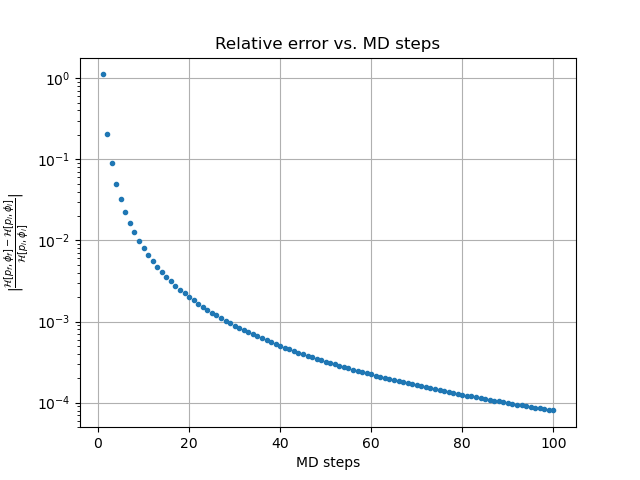
\includegraphics[width = .8\linewidth]{leapfrog_conv.png}
    \caption{Relative error in the energy vs. MD steps}
    \label{fig:lf_conv}
\end{figure}

\end{enumerate}

\end{document}